\documentclass[article]{beamer}
\usefonttheme{serif}
\usepackage{subcaption}

\usepackage[spanish]{babel}
\usepackage{academicons}
\usepackage{amsfonts, amsmath, amssymb, bm}
\usepackage{calc, calrsfs}
\usepackage{fancybox}
\usepackage{graphicx}
\usepackage{hyperref}
\usepackage{latexsym}
\usepackage{listings}
\usepackage{mathpazo, palatino}
\usepackage{multicol}
\usepackage{pifont}
\usepackage{tabularx}
\usepackage{sidecap}
\let\counterwithout\relax
\let\counterwithin\relax
\usepackage{subfigure}
\usepackage{tikz}
\usepackage{times}
\usepackage{wrapfig}
\usepackage{xcolor}
\usetheme{Warsaw}
\RequirePackage{caption}
\setbeamertemplate{background}{
\includegraphics[scale=0.45]{shields/shield-bg.pdf}}
\setbeamertemplate{bibliography item}[text]
\setbeamertemplate{blocks}[rounded][shadow]
\setbeamertemplate{caption}[numbered]
\setbeamertemplate{footline}
{
\leavevmode
\hbox{
   \begin{beamercolorbox}[wd=0.45\paperwidth,ht=2.25ex,dp=1ex,center]{author in head/foot}
     \usebeamerfont{author in head/foot}\textcolor{white}{\insertshortauthor}
   \end{beamercolorbox}

   \begin{beamercolorbox}[wd=0.45\paperwidth,ht=2.25ex,dp=1ex,center]{title in head/foot}
     \usebeamerfont{title in head/foot}\textcolor{vino}{\insertshorttitle}
   \end{beamercolorbox}

   \begin{beamercolorbox}[wd=0.1\paperwidth,ht=2.25ex,dp=1ex,center]{date in head/foot}
     \usebeamerfont{date in head/foot}\textcolor{vino}{\insertframenumber{} / \inserttotalframenumber}
   \end{beamercolorbox}
}
}
\setbeamertemplate{section in toc}[ball unnumbered]
\setbeamertemplate{subsection in toc}[ball unnumbered]

\definecolor{vino}{RGB}{95,26,31} % wine
\definecolor{dred}{RGB}{139,0,0} % dark red
\definecolor{cream}{RGB}{233, 227, 208} % cream
\definecolor{grisclaro}{HTML}{EAEDEF} %Gris claro
\definecolor{grisoscuro}{HTML}{7F9297} %Gris oscuro

\captionsetup[figure]{labelfont={color=dred,scriptsize}}
\setbeamercolor{block title}{bg=cream,fg=dred}
\setbeamercolor{footline}{bg=cream}
\setbeamercolor{frametitle}{bg=cream,fg=vino}
\setbeamercolor{item projected}{fg=white}
\setbeamercolor{section in toc}{fg=vino}
\setbeamercolor{subsection in toc}{fg=vino}
\setbeamercolor{structure}{fg=cream}
\setbeamercolor{section in head/foot}{fg=white,bg=vino}
\setbeamercolor{subsection in head/foot}{fg=vino}
\setbeamercolor{title}{bg=cream,fg=vino}

\setbeamerfont{frametitle}{size=\large}


\newcommand{\imageref}[1]{%
  \vfill
  \tiny Fuente: #1%
}

\thispagestyle{empty}
\title{Del entrelazamiento EPR al impacto industrial:}
\author{Samuel Paredes}
\institute{Mecánica Cuántica Avanzada\\
    \vspace{0.3cm}

    Programa Académico de Física\\
    \vspace{0.3cm}
    Facultad de Ciencias Matemáticas y Naturales}
\date{\vfill\scriptsize{\textit{\today}}}


\begin{document}
\nocite{*}  % <--- ESTA LÍNEA ES CLAVE

\begin{frame}
  \titlepage
\end{frame}

\section{Motivación}

\begin{frame}{Contexto histórico}

\begin{itemize}
\item 1900: Planck → cuantización de la energía
\item 1905: Einstein → cuantos de luz
\item 1913: Bohr → niveles atómicos
\item 1925–1926: formulación de la mecánica cuántica
\end{itemize}

\end{frame}

%------------------------------------------------

\begin{frame}{Consolidación de la teoría}

\begin{itemize}
\item 1925: Heisenberg → mecánica matricial
\item 1926: Schrödinger → ecuación de onda
\item 1926: Born → interpretación probabilística
\item 1927: Bohr → complementariedad
\end{itemize}

\end{frame}

%------------------------------------------------

\begin{frame}{Debate sobre la realidad}

\begin{itemize}
\item 1927: Congreso Solvay → Bohr vs Einstein
\item Problema: realidad vs medición
\item ¿La teoría es completa?
\end{itemize}

\end{frame}

%------------------------------------------------

\begin{frame}{Paradoja EPR}

\begin{itemize}
\item 1935: Einstein, Podolsky, Rosen
\item Argumento: la teoría es incompleta
\item Introducen el problema del entrelazamiento
\item Bohr responde → defensa de Copenhague
\end{itemize}

\end{frame}

\section{La Escuela de Copenhague}

\begin{frame}
\frametitle{La escuela de Copenhague}

\begin{itemize}
\item Interpretación dominante de la mecánica cuántica
\item La función de onda describe el conocimiento del sistema
\item El resultado de una medición no existe antes de medir
\item La realidad física depende del proceso de medición
\end{itemize}

\end{frame}

%------------------------------------------------

\begin{frame}
\frametitle{Escuela de Copenhague}

\begin{center}
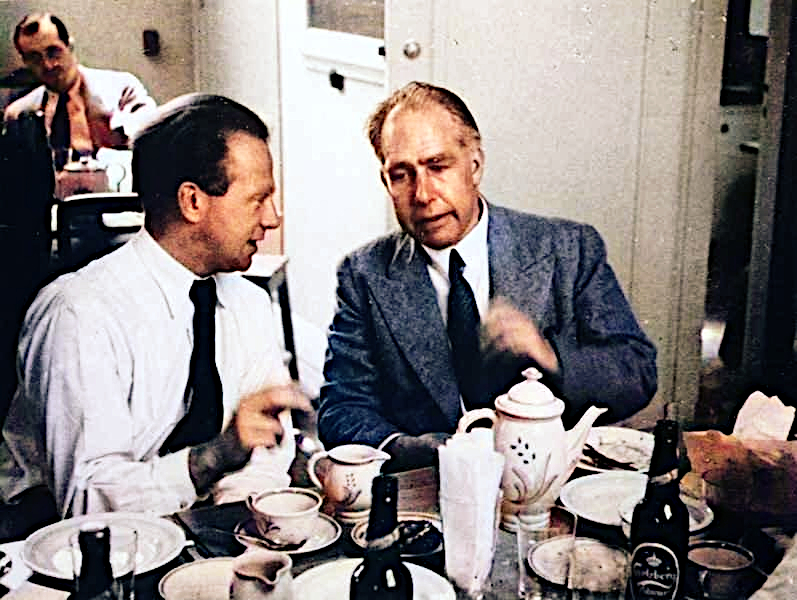
\includegraphics[width=0.8\textwidth]{images/copenhague.jpg}
\end{center}

\end{frame}

%------------------------------------------------

\section{EPR}

\begin{frame}
\frametitle{Artículo EPR (1935)}

\begin{itemize}
\item Einstein, Podolsky y Rosen publican:
\item ``Can Quantum-Mechanical Description of Physical Reality Be Considered Complete?''
\item Proponen un experimento mental
\item Concluyen que la mecánica cuántica podría ser incompleta
\end{itemize}

\end{frame}

\begin{frame}
\frametitle{Artículo original EPR}

\begin{center}
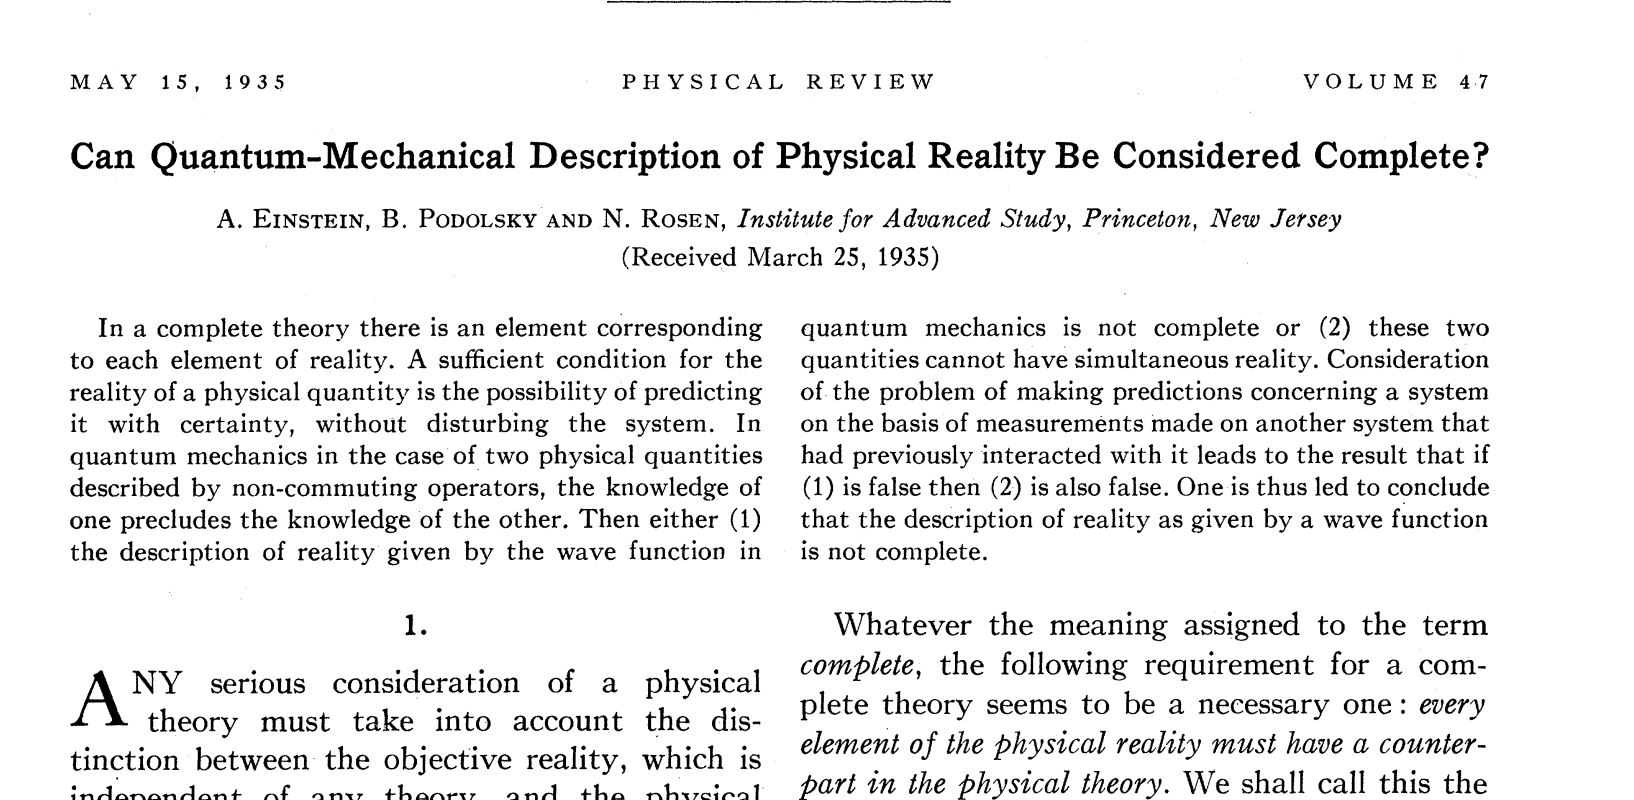
\includegraphics[width=1.1\textwidth]{images/eprpaper.jpg}
\end{center}

\end{frame}

\begin{frame}
\frametitle{Niels Bohr}

\begin{columns}

\column{0.55\textwidth}

\textbf{Niels Bohr (1885--1962)}

\begin{itemize}
\item Físico teórico danés.
\item Desarrolló el modelo cuántico del átomo (1913).
\item Figura central en el desarrollo de la mecánica cuántica.
\item Fundador de la interpretación de Copenhague.
\item Premio Nobel de Física en 1922.
\end{itemize}


\column{0.45\textwidth}
\begin{center}
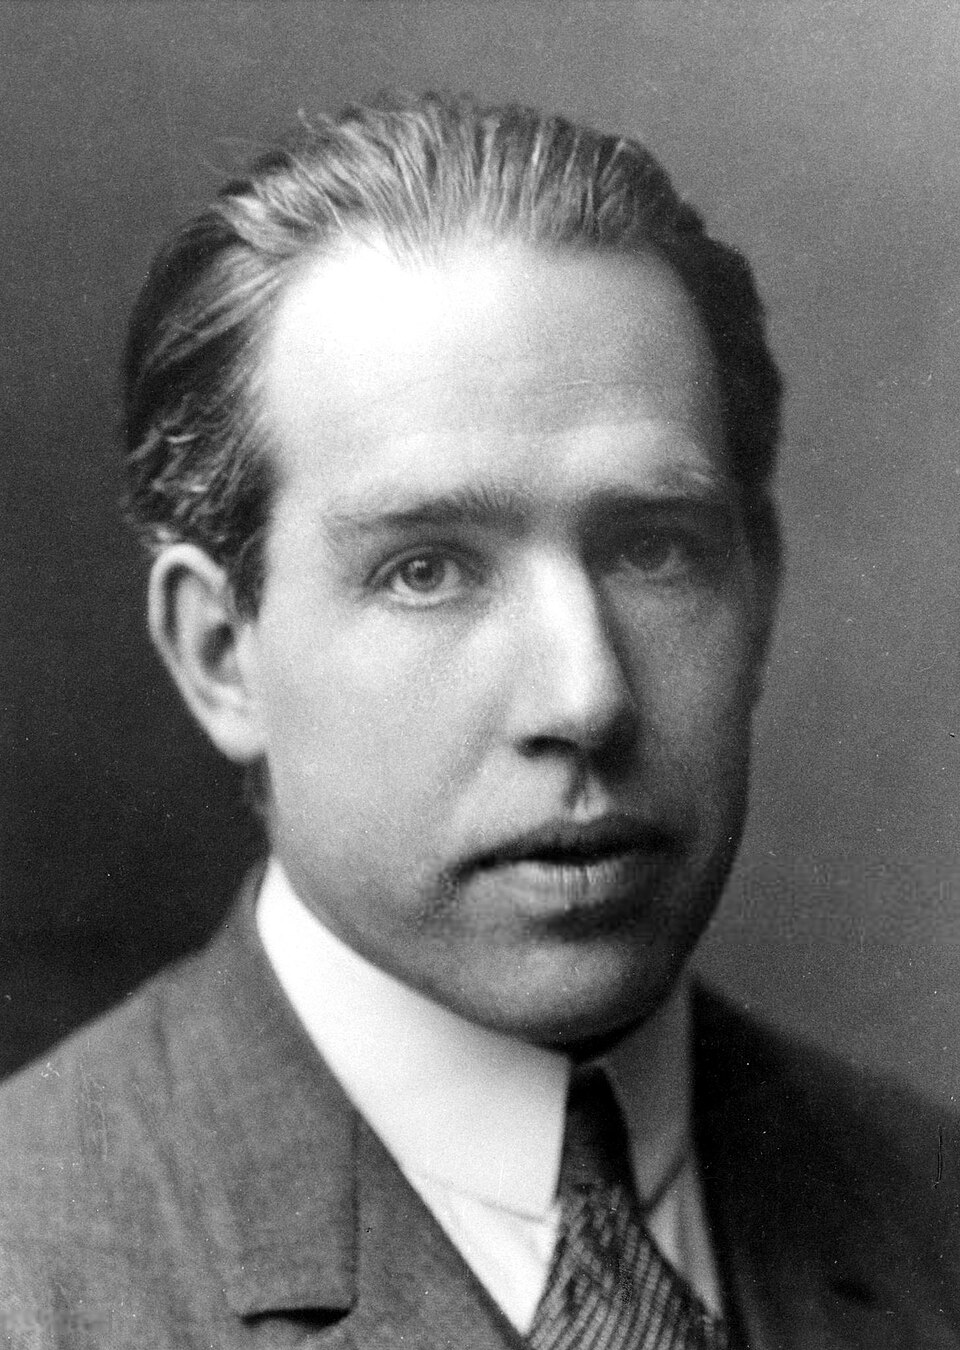
\includegraphics[width=\textwidth]{images/bohr.jpg}
\end{center}


\end{columns}

\end{frame}

\begin{frame}
\frametitle{Respuesta de Bohr a EPR}

\begin{center}
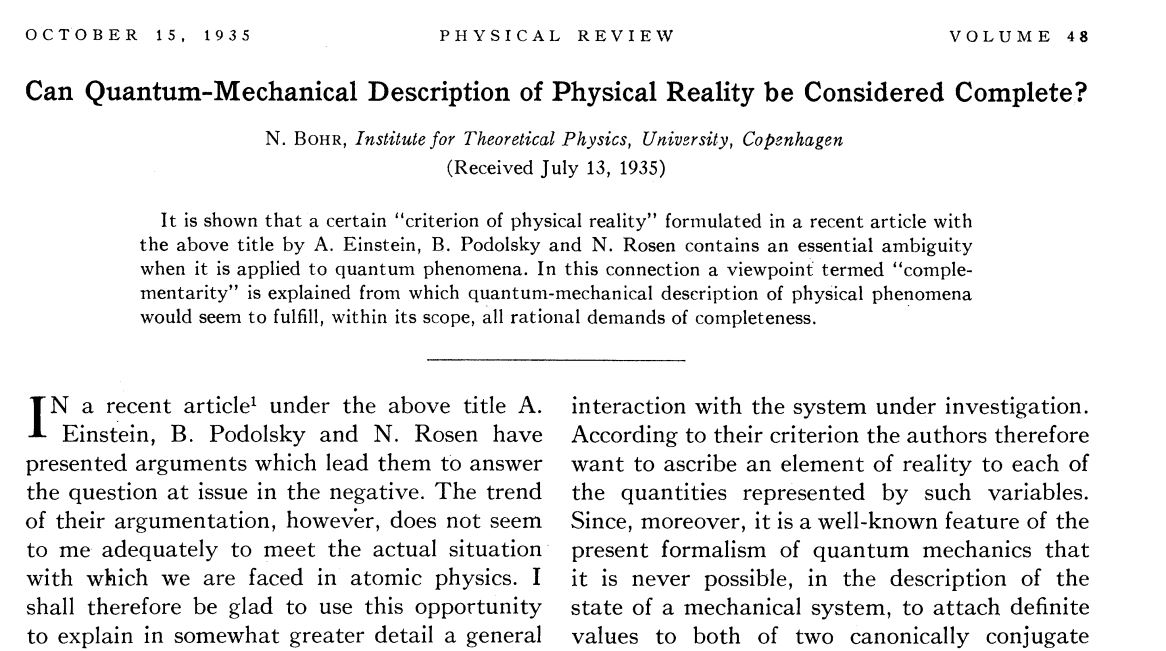
\includegraphics[width=1\textwidth]{images/paper_bohr.JPG}
\end{center}

\end{frame}


\begin{frame}{Einstein vs la Cuántica}
    \begin{figure}
        \centering
        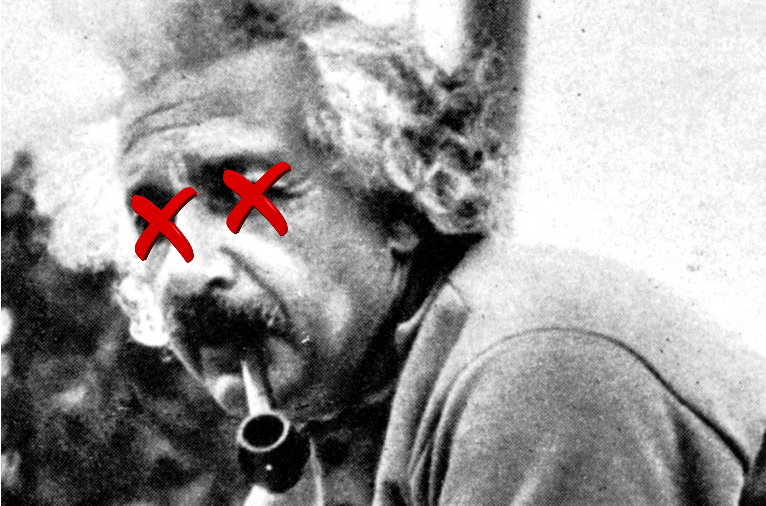
\includegraphics[width=1\linewidth]{images/einsteinnojado.png}
    \end{figure}
\end{frame}

\begin{frame}
\frametitle{Experimento mental: Alice y Bob}

\begin{itemize}
\item Dos observadores separados espacialmente
\item Cada uno mide una partícula
\item Las mediciones se realizan en diferentes direcciones
\end{itemize}

\end{frame}


\begin{frame}
\frametitle{Artículo original EPR}

\begin{center}
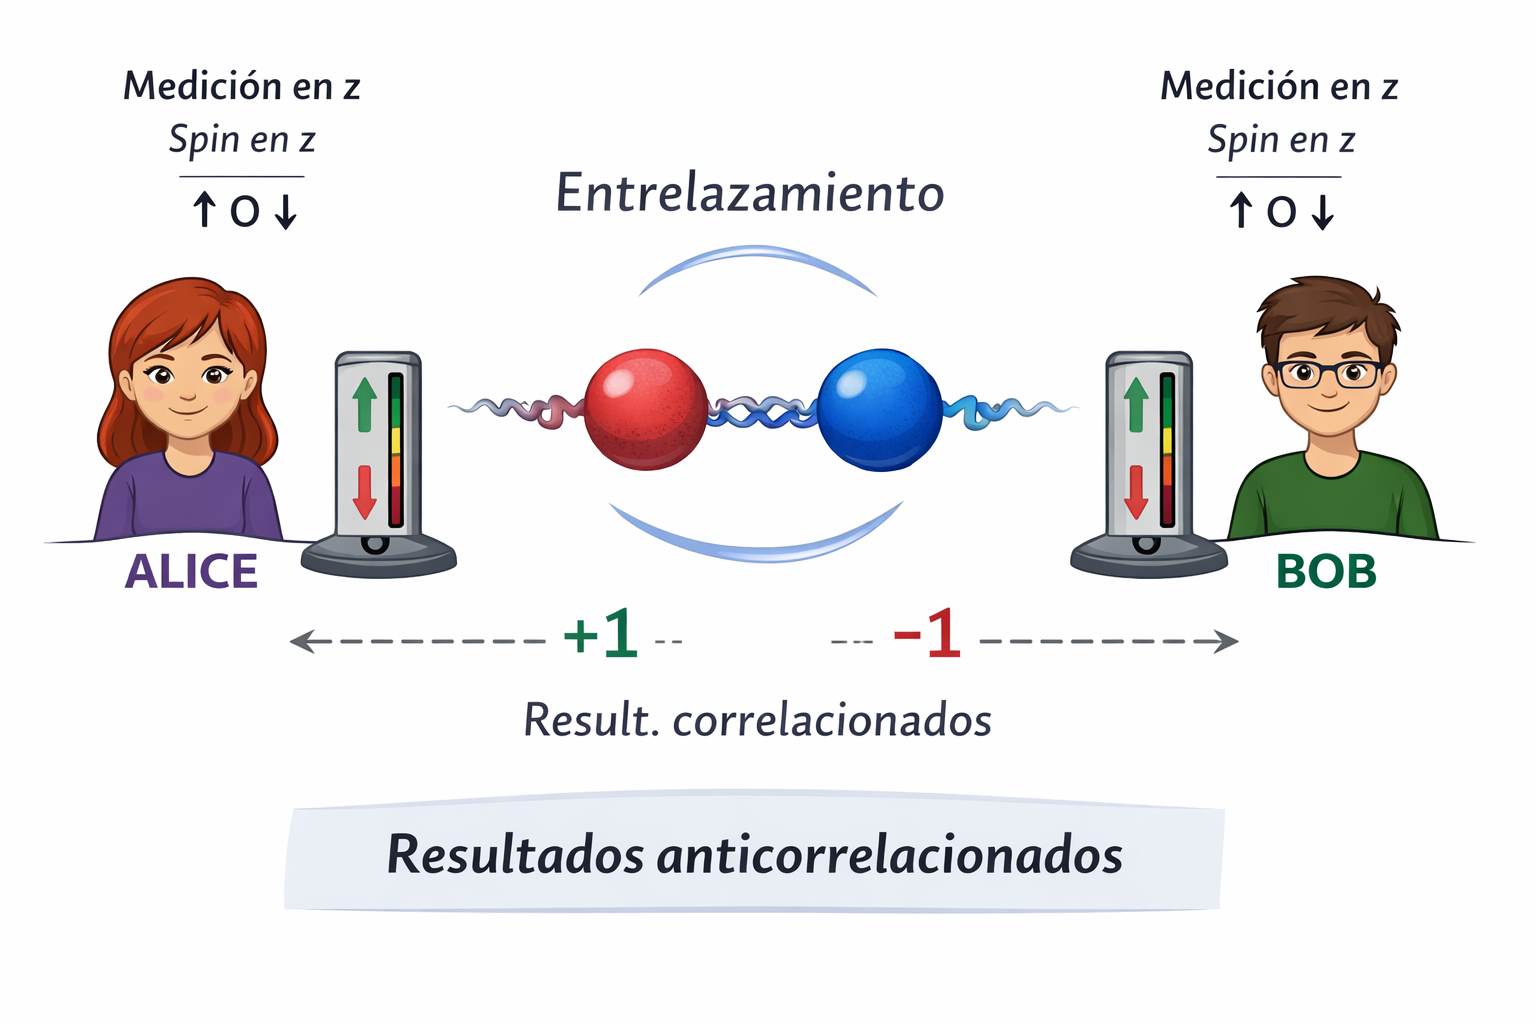
\includegraphics[width=1\textwidth]{images/alicebob.png}
\end{center}

\end{frame}


%------------------------------------------------

\begin{frame}
\frametitle{Estado singlete}

\[
|\psi^{-}\rangle =
\frac{1}{\sqrt{2}}
(|\uparrow\rangle |\downarrow\rangle -
|\downarrow \rangle |\uparrow\rangle)
\]

\begin{itemize}
\item Espín total = 0
\item Correlaciones perfectas entre partículas
\end{itemize}

\end{frame}



%------------------------------------------------
\begin{frame}
\frametitle{Albert Einstein}

\begin{columns}

\column{0.45\textwidth}
\begin{center}
\includegraphics[width=\textwidth]{images/einstein.jpg}
\end{center}

\column{0.55\textwidth}

\textbf{Albert Einstein (1879--1955)}

\begin{itemize}
\item Físico teórico alemán.
\item Desarrolló la teoría de la relatividad especial y general.
\item Premio Nobel de Física en 1921 por el efecto fotoeléctrico.
\item Crítico de la interpretación de Copenhague de la mecánica cuántica.
\item Coautor del artículo EPR (1935).
\end{itemize}

\end{columns}

\end{frame}

%------------------------------------------------

\begin{frame}
\frametitle{Boris Podolsky}

\begin{columns}

\column{0.55\textwidth}

\textbf{Boris Podolsky (1896--1966)}

\begin{itemize}
\item Físico teórico ruso-estadounidense.
\item Trabajó en mecánica cuántica y física nuclear.
\item Profesor en la Universidad de Princeton.
\item Colaborador de Einstein.
\item Coautor del artículo EPR sobre la incompletitud de la mecánica cuántica.
\end{itemize}

\column{0.45\textwidth}
\begin{center}
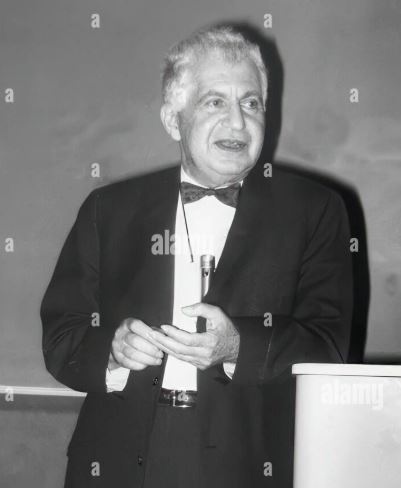
\includegraphics[width=\textwidth]{images/podolsky.jpg}
\end{center}



\end{columns}

\end{frame}

%------------------------------------------------

\begin{frame}
\frametitle{Nathan Rosen}

\begin{columns}

\column{0.45\textwidth}
\begin{center}
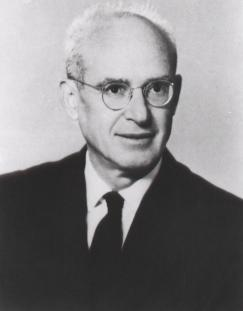
\includegraphics[width=\textwidth]{images/rosen.jpg}
\end{center}

\column{0.55\textwidth}

\textbf{Nathan Rosen (1909--1995)}

\begin{itemize}
\item Físico teórico israelí-estadounidense.
\item Trabajó en relatividad general y teoría cuántica.
\item Colaborador cercano de Einstein.
\item Coautor del artículo EPR (1935).
\item Contribuyó al estudio de los puentes Einstein--Rosen.
\end{itemize}

\end{columns}

\end{frame}


%------------------------------------------------

%------------------------------------------------

\begin{frame}
\frametitle{Elemento de realidad (EPR)}

Definición propuesta en el artículo de 1935:

\begin{itemize}
\item Si es posible predecir con certeza el valor de una magnitud física
\item sin perturbar el sistema
\item entonces existe un elemento de realidad asociado a esa magnitud
\end{itemize}

\begin{itemize}
\item Supone que las propiedades físicas existen antes de la medición
\item La teoría debe describir todos los elementos de la realidad
\end{itemize}

\end{frame}


%------------------------------------------------

\begin{frame}
\frametitle{Realismo y localidad}

\begin{itemize}
\item Realismo: las propiedades físicas existen antes de medir
\item Localidad: ninguna influencia puede viajar más rápido que la luz
\item Supuesto clave en el argumento EPR
\end{itemize}

\end{frame}

%------------------------------------------------


%------------------------------------------------


\begin{frame}{Variables ocultas}

Cada sistema está descrito por una variable oculta \(x\).

\[
A = A(x)
\]

El resultado está completamente determinado por \(x\).

\end{frame}


\begin{frame}{Distribución estadística}

No conocemos \(x\), por lo que usamos una distribución:

\[
\rho(x)
\]

Describe la probabilidad de cada estado oculto.

\end{frame}


\begin{frame}{Valor esperado}

El promedio de un observable es:

\[
\langle A \rangle = \int dx \, \rho(x)\, A(x)
\]

La teoría debe reproducir la mecánica cuántica:

\[
\langle A \rangle_{\text{HVT}} = \langle A \rangle_{\text{QM}}
\]

\end{frame}

\section{Problema de la Macroobjetivación}

\begin{frame}{Cadena de von Neumann}

La ecuación de Schrödinger es lineal.

\[
|\chi_0\rangle |\phi_1\rangle \rightarrow |\chi_1\rangle |\phi_1\rangle
\]

\[
|\chi_0\rangle |\phi_2\rangle \rightarrow |\chi_2\rangle |\phi_2\rangle
\]

\end{frame}


\begin{frame}{Superposición y Evolución lineal}

Si el sistema está en superposición:

\[
a|\phi_1\rangle + b|\phi_2\rangle
\]

\[
|\chi_0\rangle (a|\phi_1\rangle + b|\phi_2\rangle)
\]

Por linealidad:

\[
|\chi_0\rangle (a|\phi_1\rangle + b|\phi_2\rangle)
\rightarrow
a|\chi_1\rangle|\phi_1\rangle + b|\chi_2\rangle|\phi_2\rangle
\]


\end{frame}


\begin{frame}{Conclusión}

El aparato también entra en superposición.

\[
a|\chi_1\rangle|\phi_1\rangle + b|\chi_2\rangle|\phi_2\rangle
\]

Cadena de sistemas entrelazados → cadena de von Neumann.

\end{frame}

\begin{frame}
\frametitle{El gato de Schrödinger}


\begin{itemize}
\item Un sistema cuántico está en superposición
\item Un aparato mide una propiedad del sistema
\item El resultado controla la liberación de veneno
\end{itemize}

\begin{itemize}
\item Si el veneno se libera → el gato muere
\item Si no se libera → el gato vive
\end{itemize}

Según la evolución cuántica:

\[
|\text{gato}\rangle =
a|\text{vivo}\rangle + b|\text{muerto}\rangle
\]

\begin{itemize}
\item Superposición de dos estados macroscópicos
\end{itemize}

\end{frame}


\begin{frame}
\frametitle{El gato de Schrödinger}

\begin{center}
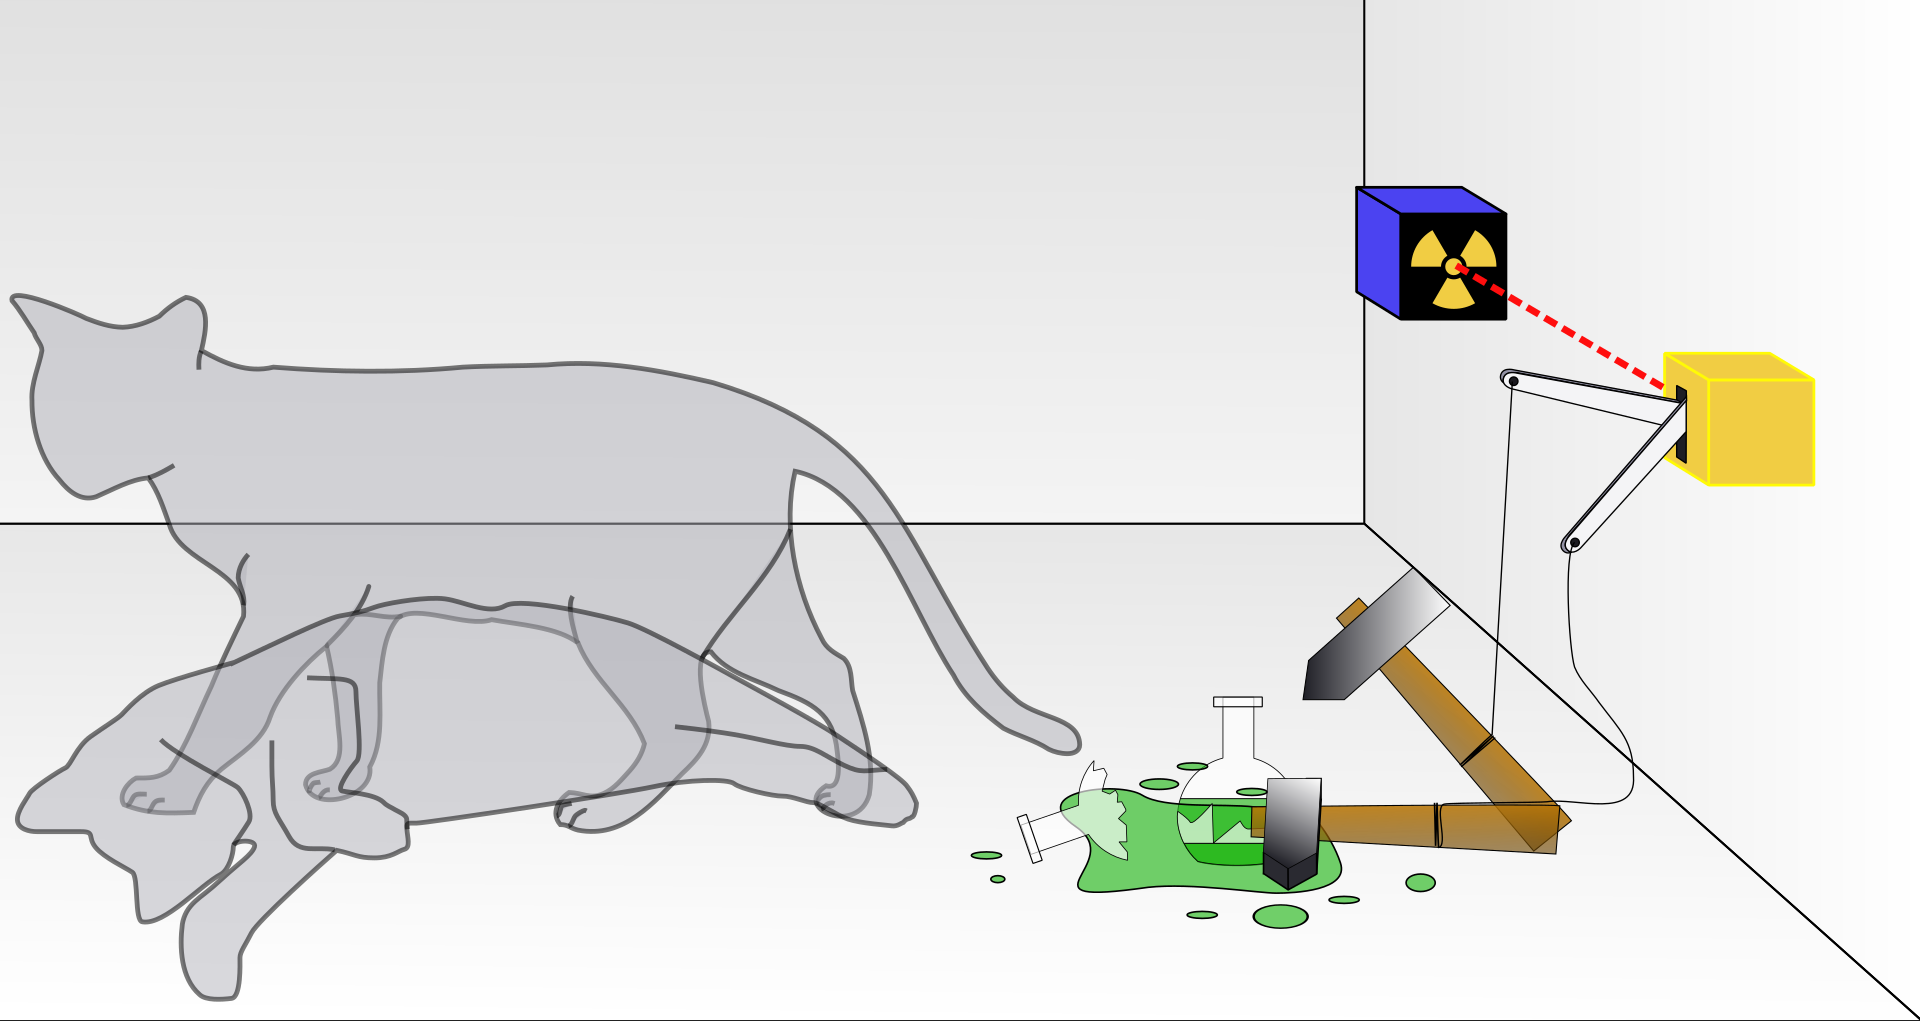
\includegraphics[width=1\textwidth]{images/gato.png}
\end{center}

\end{frame}

%------------------------------------------------


\begin{frame}
\frametitle{LHV}

\begin{itemize}
\item Local Hidden Variables
\item Variables ocultas determinan los resultados
\item Intento de restaurar realismo y localidad
\end{itemize}

\end{frame}

%------------------------------------------------

\begin{frame}
\frametitle{Local Realistic Theory}

\begin{itemize}
\item Supone simultáneamente:
\begin{itemize}
\item realismo
\item localidad
\end{itemize}
\item Base de las desigualdades de Bell
\end{itemize}

\end{frame}

%------------------------------------------------

\section{Desigualdades de Bell}


\begin{frame}{Desigualdades de Bell}

Sistema: dos partículas entrelazadas

\[
A_a , \; B_b = \pm 1
\]

\[
C(a,b)=\langle \psi_0 | (\sigma_1\cdot a)(\sigma_2\cdot b)|\psi_0\rangle
\]

\[
C(a,a)=-1
\]

\end{frame}


\begin{frame}{Variables ocultas}

\[
C(a,b)=\int_X A_a(x)\,B_b(x)\,\rho(x)\,dx
\]

\[
\int_X \rho(x)dx = 1
\]

\[
A_a(x)=-B_a(x)
\]

\end{frame}


\begin{frame}{Derivación}
Recordando
\[
A,B=\pm1
\]
Entonces
\[
|C(a,b)-C(a,c)|
=
\left|
\int_X
A_a(x)A_b(x)[1-A_b(x)A_c(x)]\rho(x)dx
\right|
\]

\[
|C(a,b)-C(a,c)|
\le
1+C(b,c)
\]

Teoría local realista

\end{frame}



\begin{frame}{Desigualdad CHSH}
Forma experimental de las desigualdades de Bell

\[
|C(a,b)-C(a,c)|
+
C(b',b)
+
C(b',c)
\le 2
\]

\[
S=
|C(a,b)-C(a,b')|
+
|C(a',b')+C(a',b)|
\le 2
\]

\end{frame}


\begin{frame}{Teorema de Fine}

Teoría determinista

\[
\Longleftrightarrow
\]

Teoría probabilística local

\end{frame}


\begin{frame}{Teorema de Fine}
    \begin{center}
        % Ajusta el ancho (width) según necesites
        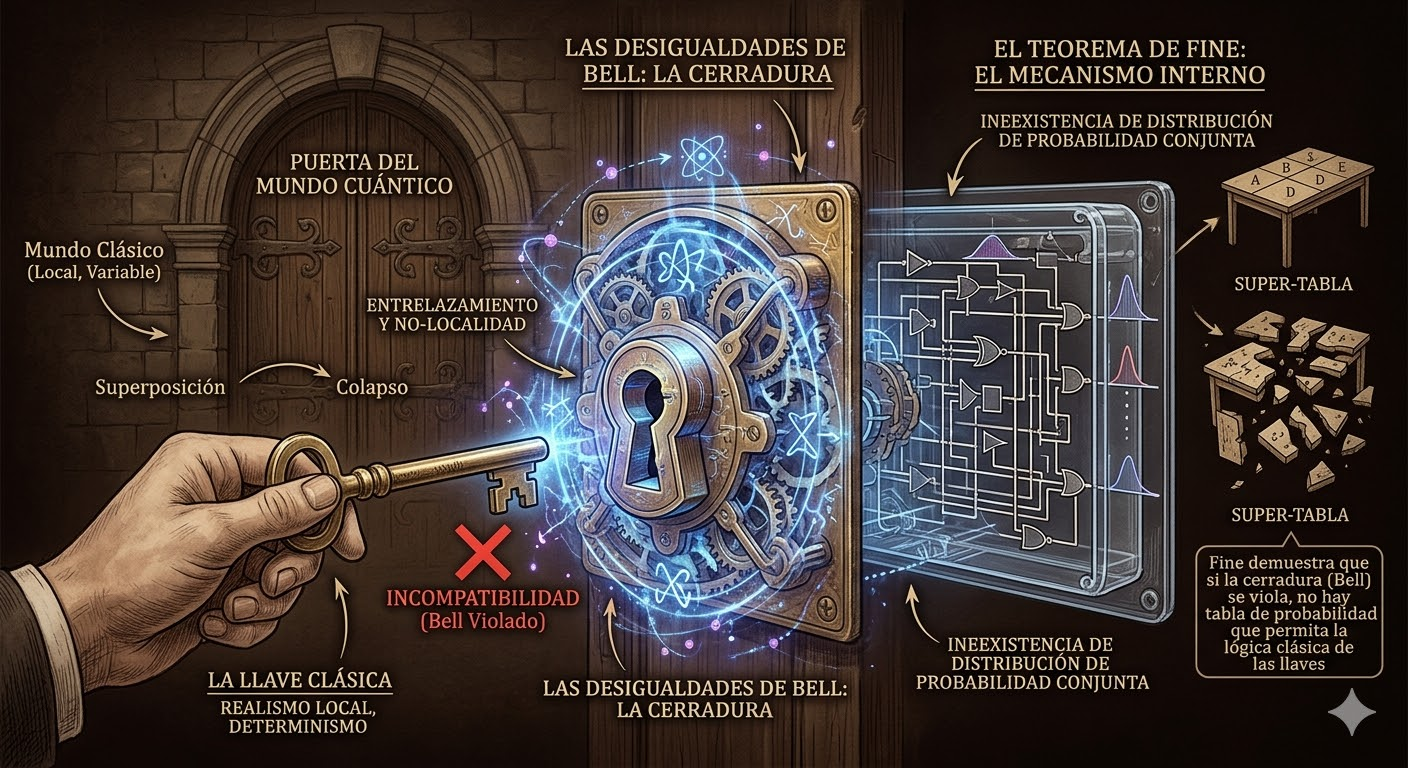
\includegraphics[width=1\textwidth]{images/teoremadefine.jpg}
    \end{center}
\end{frame}
%------------------------------------------------
\begin{frame}{Estados de Werner}

Mezcla de estado entrelazado y estado mixto:

\[
\rho_W = p\,|\psi^-\rangle\langle \psi^-| + (1-p)\frac{I}{4}
\]

\begin{itemize}
\item Entrelazados si \(p > \frac{1}{3}\)
\item Violan Bell solo si \(p > \frac{1}{\sqrt{2}}\)
\end{itemize}

\end{frame}
%------------------------------------------------

\begin{frame}
\frametitle{Entropía de von Neumann}

\[
S(\rho)=-Tr(\rho \ln \rho)
\]

Mide la información cuántica de un sistema.

\end{frame}

%------------------------------------------------
%------------------------------------------------

\begin{frame}
\frametitle{Entropía de entrelazamiento}

Para el estado singlete

\[
S(\rho_A)=\ln 2
\]

Indica entrelazamiento máximo.

\end{frame}

\begin{frame}{Experimento de Entrelazamiento}
    \begin{figure}
        \centering
        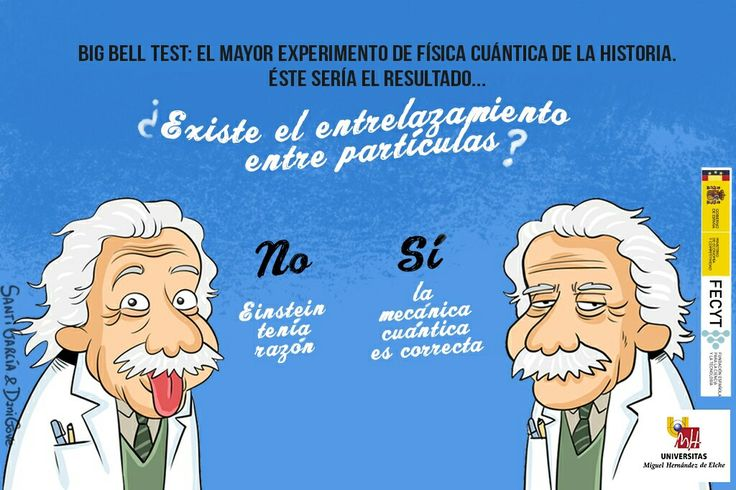
\includegraphics[width=1\linewidth]{images/expermento-eistein.jpg}
    \end{figure}
\end{frame}


\begin{frame}
\frametitle{Sistemas de Fotones Entrelazados}

\begin{itemize}
    \item Ventajas de los fotones: Facilidad de manipulacion y deteccion.
    \item Generacion (decadas de los 70 y 80): Decaimiento atomico en cascada o de positronio.
    \item Estados de polarizacion (H: horizontal, V: vertical):
\end{itemize}

\[
|\Phi^+\rangle = \frac{|H\rangle|H\rangle + |V\rangle|V\rangle}{\sqrt{2}} \quad \text{(Decaimiento atomico J = 0 to 1 to 0)}
\]

\[
|\Psi^-\rangle = \frac{|H\rangle|V\rangle - |V\rangle|H\rangle}{\sqrt{2}} \quad \text{(Decaimiento de positronio)}
\]

\end{frame}

\end{frame}

\begin{frame}{Experimento Bell}
\begin{figure}
    \centering
    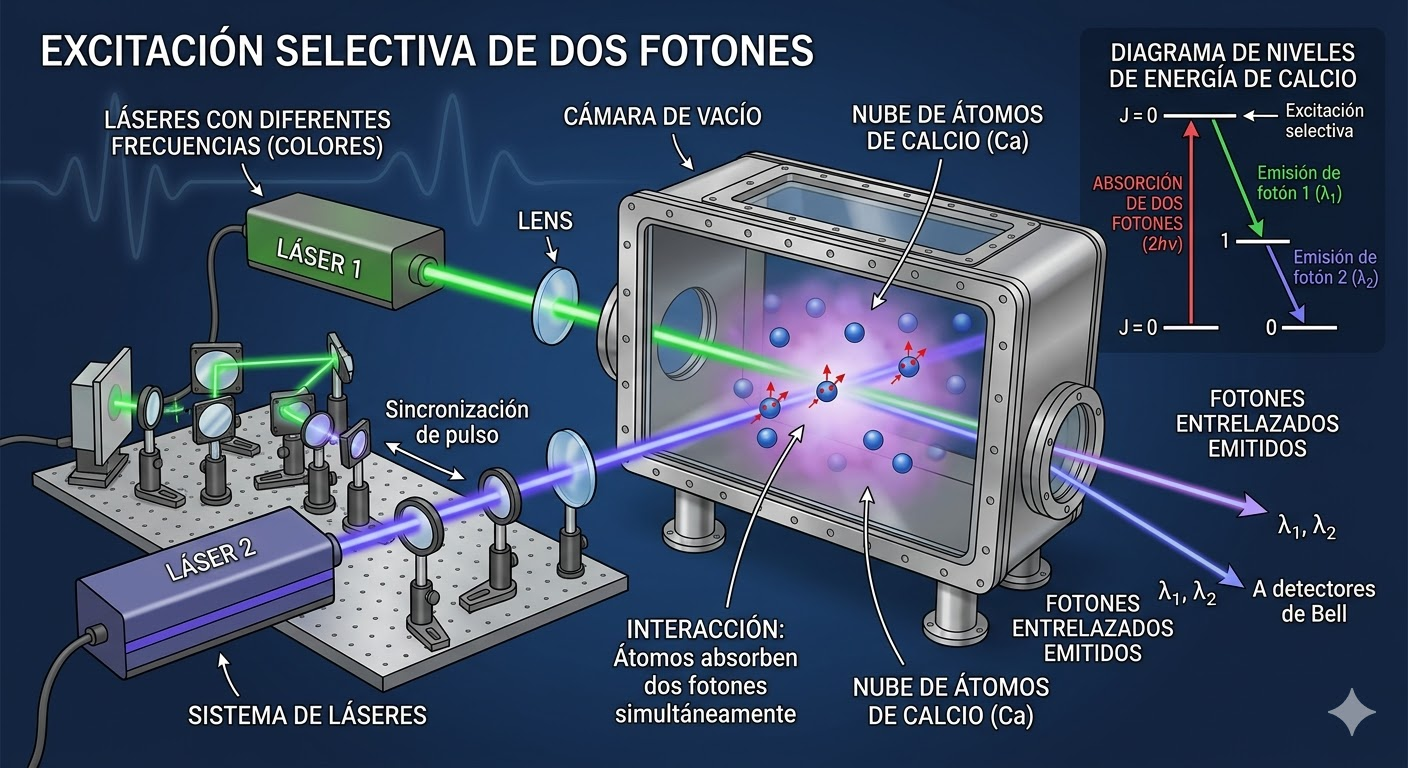
\includegraphics[width=1\linewidth]{images/bombardeo.jpg}
\end{figure}
    
\end{frame}



\begin{frame}
\frametitle{Operadores y Probabilidades de Coincidencia}

\begin{itemize}
    \item Operador de aniquilacion con polarizacion en angulo $\theta$:
\end{itemize}

\[
a_\theta = a_H \cos(\theta) + a_V \sin(\theta)
\]

\begin{itemize}
    \item Probabilidades de deteccion conjunta (coincidencias):
\end{itemize}

\[
P(\theta_1, \theta_2) = \frac{1}{2} \cos^2(\theta_1 - \theta_2) \quad \text{(Para } |\Phi^+\rangle\text{)}
\]

\[
P(\theta_1, \theta_2) = \frac{1}{2} \sin^2(\theta_1 - \theta_2) \quad \text{(Para } |\Psi^-\rangle\text{)}
\]

\end{frame}


\begin{frame}
\frametitle{Violacion de las Desigualdades de Bell}

\begin{itemize}
    \item Los resultados experimentales permiten violar las desigualdades de Bell.
    \item Ejemplo con probabilidad de coincidencia coseno cuadrado:
    \begin{itemize}
        \item Valor de violacion maxima: R = 1.207.
    \end{itemize}
    \item Configuracion de angulos criticos:
    \begin{itemize}
        \item $\theta_1 = 67.5^\circ$
        \item $\theta_2 = 45^\circ$
        \item $\theta_1' = 22.5^\circ$
        \item $\theta_2' = 0^\circ$
    \end{itemize}
\end{itemize}

\end{frame}

\begin{frame}
\frametitle{Limitaciones: Positronio vs Cascada Atomica}

\begin{itemize}
    \item Positronio: Dificultad para seleccionar polarizacion en rayos gamma (sin polarizadores lineales).
    \item Cascada Atomica: Los fotones estan en el espectro visible.
    \item Modificacion de probabilidad por eficiencias ($\eta$):
\end{itemize}

\[
P_i(\theta) = \frac{1}{2} \eta_i f_i \epsilon_i^+
\]

\begin{itemize}
    \item Problema de deteccion (Detection Loophole): Solo se detecta una pequeña submuestra de los pares producidos.
\end{itemize}

\end{frame}


\begin{frame}
\frametitle{Premio Nobel de Fisica 2022}

\begin{itemize}
    \item Galardonados: Alain Aspect, John Clauser y Anton Zeilinger.
    \item Hito principal: Experimentos con fotones entrelazados.
    \item Contribucion clave:
        \begin{itemize}
            \item Violacion de las desigualdades de Bell.
            \item Establecimiento de la ciencia de la informacion cuantica.
        \end{itemize}
    \item Experimento:
        \begin{itemize}
            \item Generacion de pares de fotones correlacionados.
            \item Demostracion de que no existen variables ocultas locales.
            \item Validacion de la naturaleza no local de la realidad.
        \end{itemize}
\end{itemize}

\end{frame}


\begin{frame}
\frametitle{Galardonados Nobel de Fisica 2022}

\begin{figure}
    \centering
    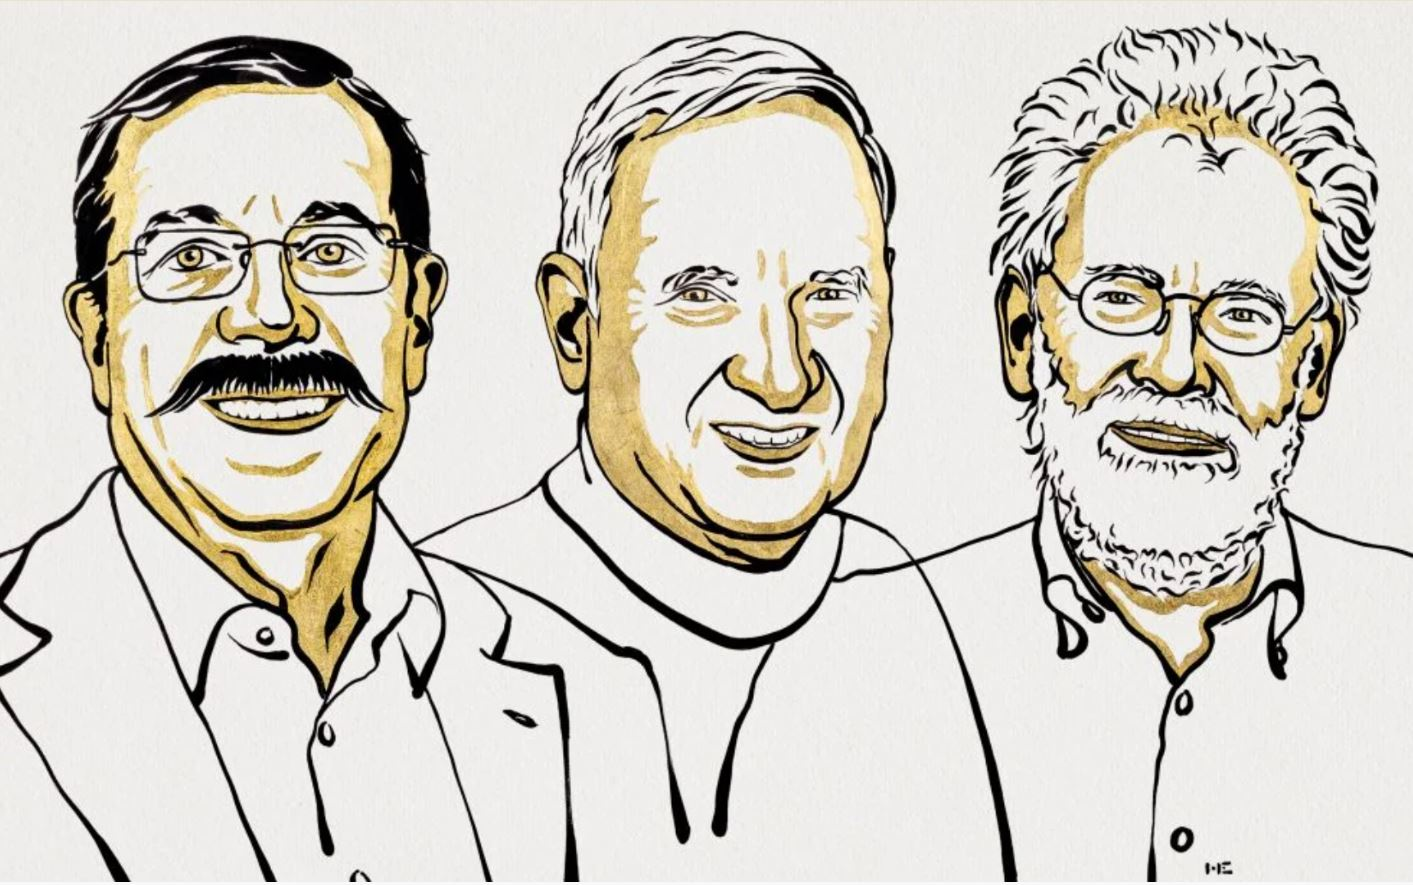
\includegraphics[width=0.8\textwidth]{images/nobel2022.JPG}
\end{figure}

\end{frame}


%------------------------------------------------

\section{Computación cuántica}

\begin{frame}
\frametitle{Qubit}

\[
|\psi\rangle = \alpha|0\rangle + \beta|1\rangle
\]

\begin{itemize}
\item Unidad de información cuántica
\item Puede existir en superposición
\item $\alpha, \beta$ son amplitudes de probabilidad
\item $|\alpha|^2 + |\beta|^2 = 1$
\end{itemize}

\end{frame}
%------------------------------------------------
\begin{frame}{Esfera de Bloch}
\begin{figure}
    \centering
    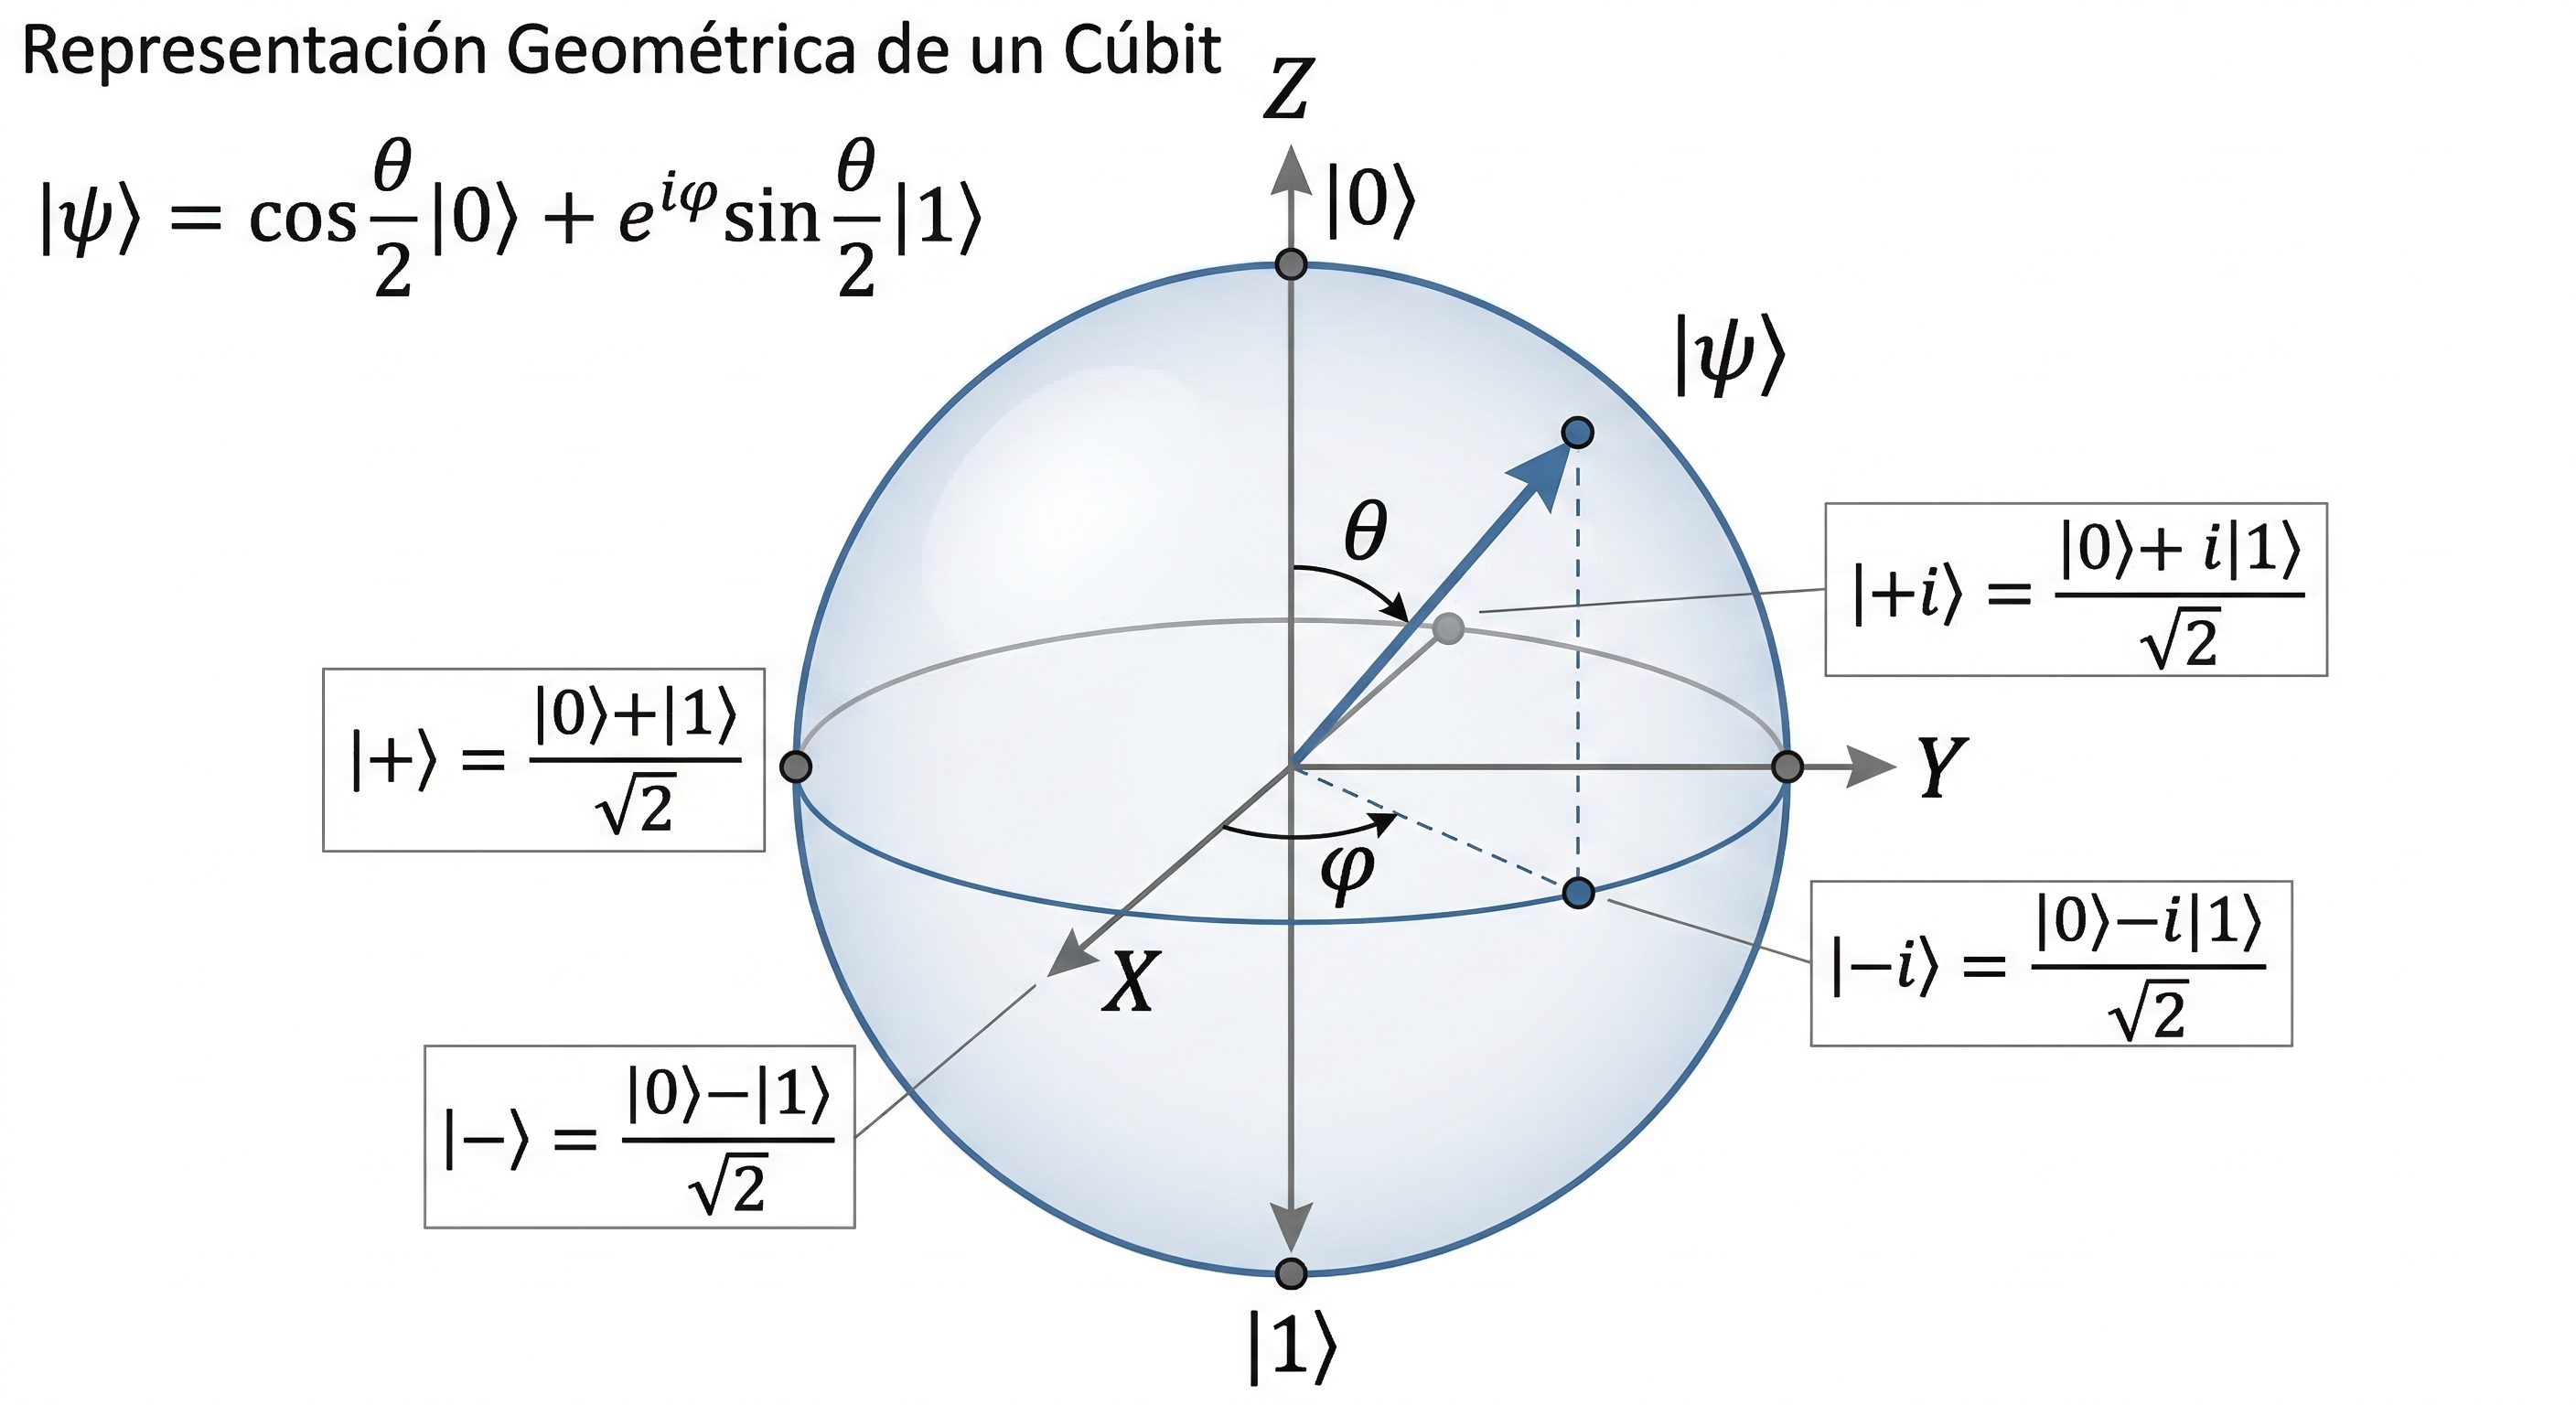
\includegraphics[width=1\linewidth]{images/esferablochj.png}
\end{figure}
    
\end{frame}
%------------------------------------------------

\begin{frame}
\frametitle{Decoherencia}

Interacción con el entorno destruye la coherencia cuántica.

El sistema pasa de

\[
|\psi\rangle
\]

a una mezcla clásica descrita por una matriz de densidad.

\end{frame}

%------------------------------------------------

\begin{frame}
\frametitle{Ejemplo}

Antes:

\[
|\psi\rangle =
\frac{1}{\sqrt{2}}(|cara\rangle+|sello\rangle)
\]

Después de la decoherencia:

\begin{itemize}
\item 50\% cara
\item 50\% sello
\end{itemize}

\end{frame}

\begin{frame}
\frametitle{Desafíos del entrelazamiento}

\begin{itemize}
\item Mantener estados entrelazados es muy difícil
\item Vulnerables a perturbaciones ambientales
\item Puede ocurrir \textbf{“muerte súbita del entrelazamiento”}
\item Superar esto es clave para computación cuántica a gran escala
\end{itemize}

\end{frame}

%-----------------------------------------------



\begin{frame}{Muerte Súbita del Entrelazamiento}


    \begin{figure}
        \centering
        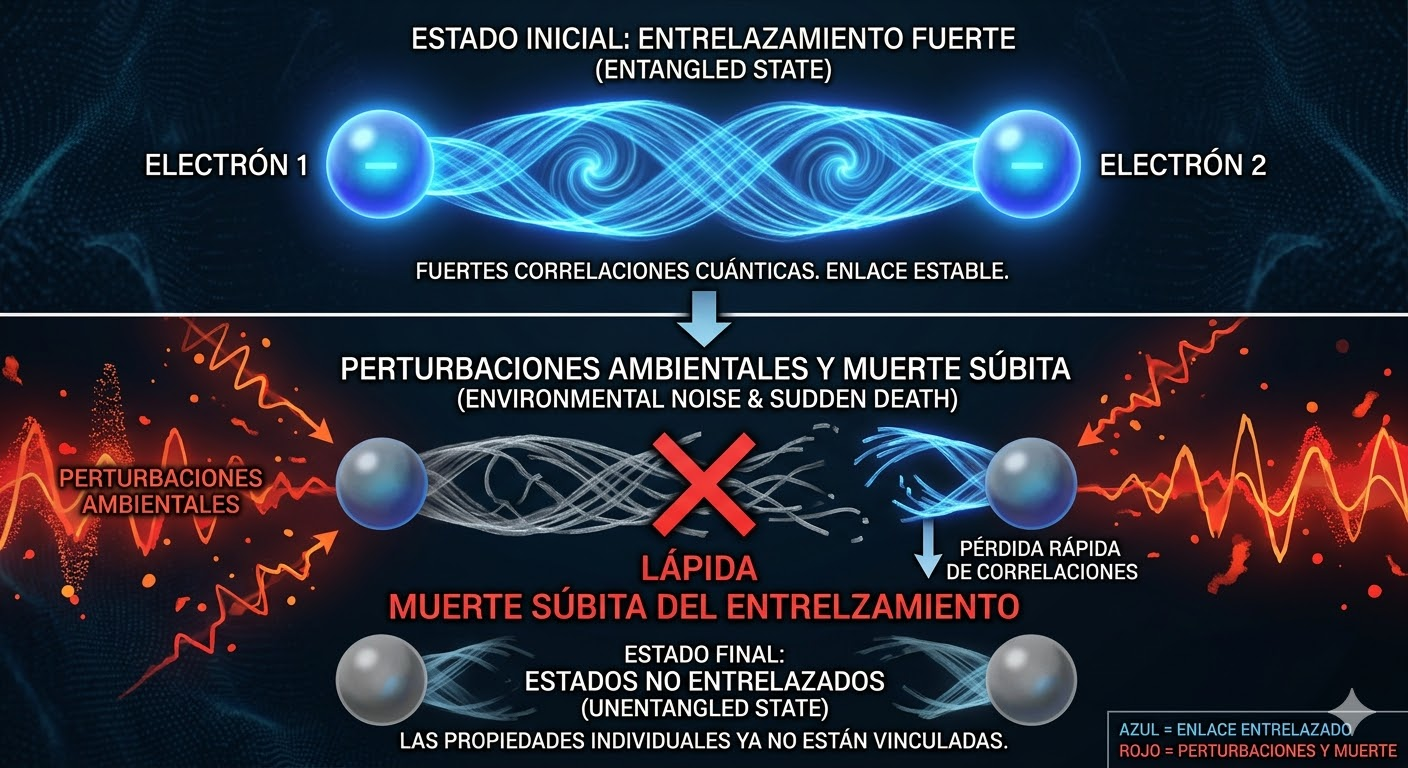
\includegraphics[width=1\linewidth]{images/muertesubita.jpg}
    \end{figure}
\end{frame}

%------------------------------------------------
\section{IA y Computación Cuántica}

\begin{frame}
\frametitle{Computación Cuántica y IA/ML}

\begin{itemize}
    \item Sinergia: Aceleración computacional y algoritmos innovadores.
    \item Mecánica Cuántica en IA:
        \begin{itemize}
            \item Eficacia del aprendizaje.
            \item Superposición y Entrelazamiento (estructuras complejas).
        \end{itemize}
    \item Hitos Clave:
        \begin{itemize}
            \item Búsqueda mejorada (inspirada en Grover).
            \item QSVM (clasificación de alta dimensión).
            \item Redes Neuronales Cuánticas (QNN).
        \end{itemize}
    \item Impacto: Entrenamiento acelerado y reconocimiento de patrones complejos.
\end{itemize}

\end{frame}
\begin{frame}{Entrelazamiento Cuántico}
    \begin{figure}
        \centering
        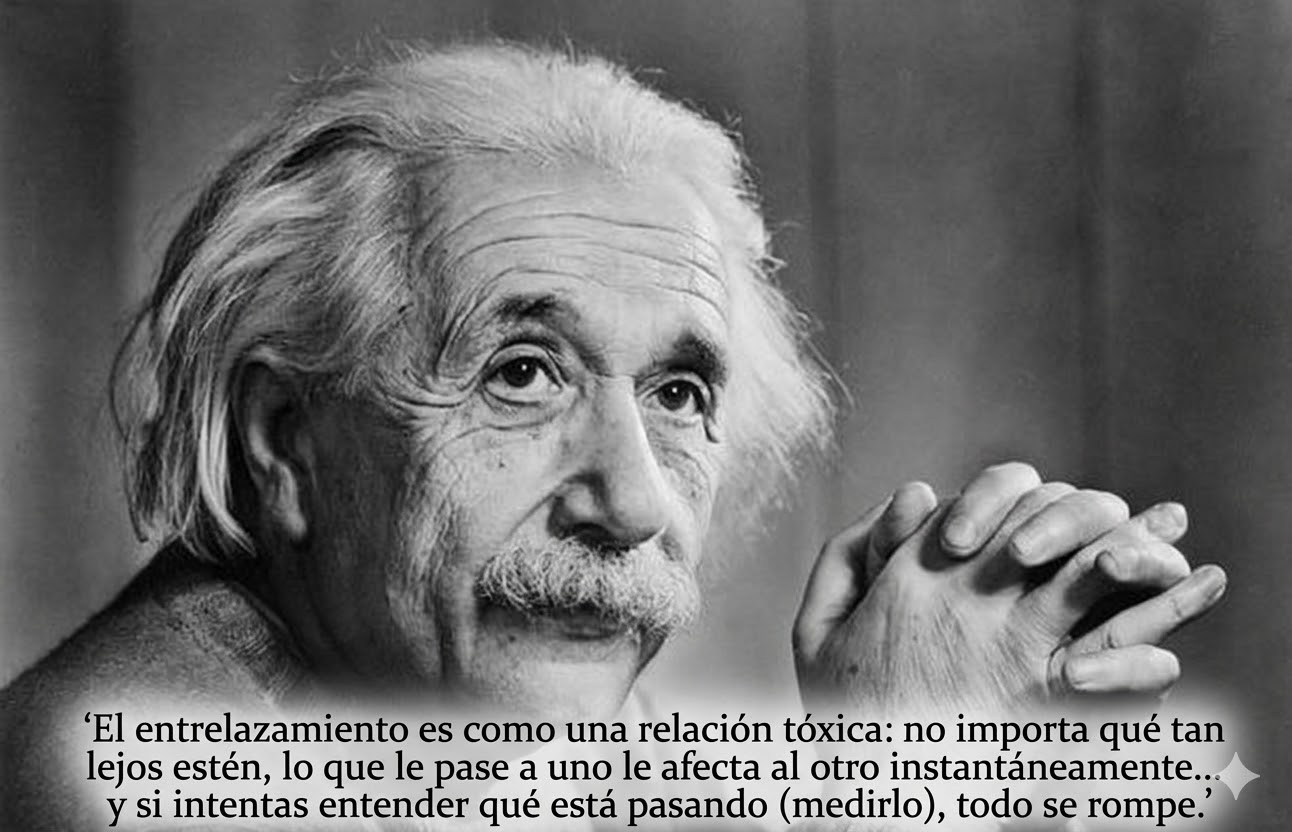
\includegraphics[width=0.9\linewidth]{images/relaciontoxica.jpg}
    \end{figure}
\end{frame}


\begin{frame}
\frametitle{Memristores Cuánticos: Potencial Numérico}

\begin{itemize}
    \item Precision de Clasificacion: Reconocimiento de imagenes.
    \item Mejora Sustancial:
        \begin{itemize}
            \item Sistemas Memristivos Clasicos: 71 %.
            \item Redes Cuanticas (Memristores): 95 %.
        \end{itemize}
    \item Fusion Clave: Paralelismo cuantico + Arquitecturas adaptativas.
\end{itemize}

\end{frame}


\begin{frame}
\frametitle{Comparacion de Investigacion en IA/ML Cuantica}

\small
\begin{tabularx}{\textwidth}{|X|X|X|}
\hline
Trabajo de Investigacion & Contribucion Clave & Mejora del Rendimiento \\ \hline
Paralelizacion cuantica & Computacion mas rapida mediante aceleracion cuantica & Exponencial en tareas complejas \\ \hline
Redes neuronales cuanticas (QNN) & Modelos de aprendizaje profundo mejorados cuanticamente & Reconocimiento de patrones mas rapido \\ \hline
Maquinas de vectores de soporte (QSVM) & Clasificacion mejorada mediante nucleos cuanticos & Aceleracion cuadratica \\ \hline
Análisis de componentes principales (QPCA) & Reduccion de dimensionalidad mas rapida & Aceleracion exponencial \\ \hline
Aprendizaje por refuerzo cuantico (QRL) & Aprendizaje mejorado en entornos dinamicos & Mejor optimizacion de politicas \\ \hline
\end{tabularx}

\end{frame}

\begin{frame}
\frametitle{Blockchain Cuantica: Entrelazamiento en el Tiempo}

\begin{itemize}
    \item Concepto: Utiliza entrelazamiento temporal para vincular bloques.
    \item Beneficios en la integridad:
        \begin{itemize}
            \item Mejora la proteccion de los datos frente a ataques.
            \item Previene modificaciones historicas de los registros.
        \end{itemize}
    \item Resultado: Registros inmutables ante la capacidad de computo cuantico.
    \item Seguridad: Garantiza la inviolabilidad del historial de la cadena.
\end{itemize}

\end{frame}

\begin{frame}
\frametitle{Contribuciones en Blockchain Cuantica (Parte 1)}

\small
\begin{tabularx}{\textwidth}{|X|X|}
\hline
Nombre del Modelo & Importancia en el Campo \\ \hline
Marco de cadena de bloques post-cuantico & Cifrado basado en reticulos y firmas hash contra amenazas cuanticas. \\ \hline
Modelo de cadena de bloques cuanticamente seguro & Distribucion de claves cuanticas para comunicacion a prueba de manipulaciones. \\ \hline
Cadena de bloques mediante entrelazamiento en el tiempo & Garantiza la inmutabilidad de los datos mediante entrelazamiento temporal. \\ \hline
Arquitectura hibrida cuantico-clasica & Combina criptografia clasica y resistente para sistemas seguros y compatibles. \\ \hline
\end{tabularx}

\end{frame}

%------------------------------------------------

\begin{frame}
\frametitle{Contribuciones en Blockchain Cuantica (Parte 2)}

\small
\begin{tabularx}{\textwidth}{|X|X|}
\hline
Nombre del Modelo & Importancia en el Campo \\ \hline
Prueba de participacion delegada cuantica (QDPoS) & Mecanismos de consenso robustos y seguros para la gobernanza. \\ \hline
Marco de autenticacion de identidad post-cuantico & Refuerza la identidad con esquemas de firma digital resistentes. \\ \hline
Sistema de criptomonedas cuanticamente seguro & Protege transacciones de activos digitales contra descifrado cuantico. \\ \hline
Modelo asistido por computacion cuantica & Mejora la velocidad y escalabilidad de la verificacion de transacciones. \\ \hline
Modelo basado en aprendizaje profundo cuantico & Optimiza la validacion y asignacion de recursos mediante ML cuantico. \\ \hline
\end{tabularx}

\end{frame}

\section{Bibliografía}

\begin{frame}[allowframebreaks]{Bibliografía}
    \footnotesize
    \bibliographystyle{unsrt}
    \bibliography{bibliography}
\end{frame}


\end{document}